\documentclass[10pt]{article}

\usepackage[a4paper,total={17cm,25cm}]{geometry}

\usepackage[fleqn]{amsmath}
\usepackage{amssymb}
\usepackage{mathrsfs}
\usepackage{amsthm}
\usepackage{dsfont}
\usepackage[mathcal]{euscript}

\usepackage{enumitem}

\usepackage{algorithm}
\usepackage{algpseudocode}

\usepackage[colorlinks=true, citecolor=blue]{hyperref}
\usepackage[capitalise]{cleveref}

\usepackage{graphicx}
\usepackage[skip=0cm, font=footnotesize, labelfont=bf, labelsep=period]{caption}
\usepackage[dvipsnames]{xcolor}

\usepackage[backend=biber, style=ieee]{biblatex}
\addbibresource{Refs.bib}
\renewcommand*{\bibfont}{\small}

\newtheorem{thm}{Theorem}[section]
\newtheorem{lem}[thm]{Lemma}
\newtheorem{cor}[thm]{Corollary}
\theoremstyle{definition}
\newtheorem{defn}{Definition}[section]
\newtheorem{exmp}{Example}[section]
\newtheorem*{rem}{Remark}

\crefname{lem}{Lemma}{Lemmas}
\crefname{thm}{Theorem}{Theorems}

\newenvironment{prf}{\noindent\textbf{Proof.}}{\hfill$\blacksquare$}

\counterwithin{equation}{section}
\newcommand\eqnum{\addtocounter{equation}{1}\tag{\arabic{section}.\arabic{equation}}}
\newcommand{\overbar}[1]{\mkern 1.5mu\overline{\mkern-1.5mu#1\mkern-1.5mu}\mkern 1.5mu}
\algnewcommand{\LineComment}[1]{\State {\color{ForestGreen} \(\triangleright\) #1}}

\DeclareMathOperator{\cov}{cov}
\DeclareMathOperator{\gp}{GP}
\DeclareMathOperator{\tr}{tr}
\DeclareMathOperator{\df}{d\!}
\DeclareMathOperator*{\argmax}{\arg\max\,}

\begin{document}

\begin{titlepage}
\begin{center}
{\Large \scshape Gaussian Processes} \\
\bigskip
H. Rahnama \\
\verb|hosein.rahnama@outlook.com|
\end{center}
\bigskip
\begin{abstract}
This is an introduction to the basics of Gaussian Processes (GP). Particulary, we are interested in their applications for regression and machine learning. The tutorial is mainly divided in two parts. In the first part, we present a step-by-step explanation of the necessary mathematics to understand GPs. For this purpose, we assume that the reader is familiar with linear algebra, probability, and multivariable calculus. In this part, we touch upon the Cholesky decomposition, the matrix inversion lemma for partitioned matrices, MultiVariate Normal (MVN) Probability Density Functions (PDF) for continuous random vectors, and three main operations assosiated with MVNs, namely sampling, conditioning, and marginalization. In the second part, we define what a GP is and learn how to do regression with GPs in the cases of noise-free and noisy data observations. Afterwards, we present a simple algorithm to do regression with GPs, investigate its time complexity and implementation. Then, we study the effect of hyperparameters of a special kernel function, well known as the Radial Basis Function (RBF), on the predictive distribution. This sets the motivation for optimizing the hyperparameters, which we shall address briefly via introducing Cross Validation (CV) and Marginal Likelihood (ML). We also talk about the methods of combining available kernels to construct new ones. Afterwards, we address a real world application of GPs for designing interactive interfaces. The paper concludes with some remarks about the connection of GPs with other models and their capability for scaling. \\[\baselineskip]
\textbf{keywords}. Gaussian Process, Multivariate Normal Distribution, Regression, Kernels, Hyperparameters.
\end{abstract}
\tableofcontents
\end{titlepage}


\section{Mathematical Preliminaries}\label{sec:1}
In the first part of this tutorial, we express the mathematics that we will employ in the second part. Let us first pay attention to a very useful matrix decomposition.
\subsection{Cholesky Decomposition}
This decomposition for Symmetric Positive Definite (SPD) matrices is in perfect analogy with the square root of a positive real number.
\begin{thm}[Cholesky Decomposition]\label{thm:chol}
Let $\mathsf{A} \in \mathbb{R}^{n,n}$ be a real square matrix. The matrix $\mathsf{A}$ is SPD if and only if there exists a non-singular lower-triangular matrix $\mathsf{L}\in \mathbb{R}^{n,n}$ such that $\mathsf{A}=\mathsf{L} \mathsf{L}^{\top}$. This is called the \textbf{Cholesky decomposition} of $\mathsf{A}$ and $\mathsf{L}$ is called the \textbf{Cholesky factor} of $\mathsf{A}$.
\end{thm}
\begin{rem}
Factoring the diagonal elements of $\mathsf{L}$ in the Cholesky decomposition of $\mathsf{A}$, we arrive at $\mathsf{A}=\bar{\mathsf{L}}\mathsf{D}\bar{\mathsf{L}}^\top$ with $\mathsf{D}$ a digonal matrix with positive entries and $\bar{\mathsf{L}}$ an invertible lower triangular matrix with ones on its diagonal. This form is unique, while the Cholesky decompositon is not. More specifically, if $\mathsf{L}$ is a Cholesky factor of matrix $\mathsf{A}$ so is $-\mathsf{L}$.
\end{rem}
From \cref{thm:chol} and the facts that $\det\mathsf{A}\mathsf{B}=\det\mathsf{A}\det\mathsf{B}$, $\det\mathsf{A}=\det\mathsf{A}^\top$, it follows quickly that
\begin{cor}
If $\mathsf{A} \in \mathbb{R}^{n,n}$  is SPD then its determinant is given by $\det\mathsf{A} = (\det\mathsf{L})^2 $.
\end{cor}
The Cholesky decomposition is numerically stable for solving symmetric positive definite linear systems of equations and is the main method of choice for computation if it is available. Below is an algorithm that remedies the computation of Cholesky decomposition. The \Cref{alg:chol} simply assumes that matrix $\mathsf{A}$ has a Cholesky decomposition and exploits the fact that
\begin{equation*}
a_{jk}  = \sum_{i=1}^{n}l_{ji}l_{ki} = 
\sum_{i=1}^{\min\{j, k\}}l_{ji}l_{ki} = 
\sum_{i=1}^{k}l_{ji}l_{ki}, 
\qquad k=1,\dots, n, \qquad j = k,\dots, n
\eqnum
\label{eq:chol}
\end{equation*}
to calculate the columns of $\mathsf{L}$ inductively. When $k=1$, we observe that 
\begin{equation*}
a_{j1} = \sum_{i=1}^{1}l_{ji}l_{1i} = l_{j1}l_{11}, \qquad j = 1,\dots, n
\eqnum
\end{equation*}
Now, considering the cases $j=1$ and $j>1$, one concludes that
\begin{align*}
l_{11} &= \sqrt{a_{11} } \\
l_{j1} &= a_{j1}/l_{11}, \qquad j=2,\dots,n,
\eqnum
\end{align*}
meaning that the first column of $\mathsf{L}$ is computed. Suppose that we have computed the first $k-1$ columns of $\mathsf{L}$ and we want to compute the $k$th column. Again, by considering the cases $j=k$ and $j>k$ in \cref{eq:chol}, we obtain the following inductive equations
\begin{alignat*}{2}
l_{kk} &= \Big(a_{kk} - \sum_{i=1}^{k-1}l_{ki}^2\Big)^{\frac{1}{2}}, && k=2,\dots,n, \\ 
l_{jk} &= \Big(a_{jk}-\sum_{i=1}^{k-1}l_{ki}l_{ji}\Big)/l_{kk}, \qquad && j = k+1,\dots, n,
\eqnum
\label{eq:chol:alg}
\end{alignat*}
where all of the terms on the right hand sides (RHS) are known according to the hypothesis of induction. Using \Cref{alg:chol}, it can be easily verified that
\begin{cor}
Time complexity of computing the Cholesky decomposition of a SPD matrix $A$ is of order $\mathcal{O}(\frac{1}{6}n^3)$.
\end{cor}
\noindent
and we also have the following result
\begin{cor}
Given the Cholesky decomposition, solving the SPD linear system $\mathsf{A}\mathbf{x}=\mathbf{b}$ reduces to solving the lower-triangular $\mathsf{L}\mathbf{y} = \mathbf{b}$ and upper-triangular $\mathsf{L}^{\top} \mathbf{x} = \mathbf{y}$  linear systems. Time complexity of solving each of these is of order $\mathcal{O}(\frac{1}{2}n^2)$.
\end{cor}

\begin{algorithm}[t]
\caption{Cholesky Decomposition}\label{alg:chol}
\hspace*{\algorithmicindent} {\scshape Input}: $\mathsf{A}$\\
\hspace*{\algorithmicindent} {\scshape Output}: $\mathsf{L}$
\begin{algorithmic}[1]
\LineComment{Initialize the first column of $\mathsf{L}$ with zeros.}
\For{$j=1$ \textbf{to} $n$}
	\State $l_{j1} = 0$;
\EndFor
\For{$k=1$ \textbf{to} $n$}
    \LineComment{Calculate $l_{kk}$.}
	\State sum = $0$;
	\For{$i=1$ \textbf{to} $k-1$}
		\State sum = sum + $l_{ki}l_{ki}$;
	\EndFor
	\State $l_{kk} = a_{kk}- \text{sum}$;
	\LineComment{Check for positive definitness.}
	\If{$l_{kk} \leq 0$}
		\State print $A$ is not positive definite;
		\State return;
    \EndIf
	\State $l_{kk} = \sqrt{l_{kk}}$;
    \LineComment{Calculate $l_{jk}$ for $j>k$.}
    \For{$j=k+1$ \textbf{to} $n$}
    	\State sum = $0$;
    	\For{$i=1$ \textbf{to} $k-1$}
    		\State sum = sum + $l_{ki}l_{ji}$;
    	\EndFor
    	\State $l_{jk}=(a_{jk}-\text{sum})/l_{kk}$;
    \EndFor
\EndFor
\end{algorithmic}
\end{algorithm}

\subsection{Matrix Inversion Lemma}
Here, we shall discuss an important lemma for inverting a partioned matrix and its imediate consequences. It will be useful in dealing with MVN PDFs. We have the following theorem.
\begin{thm}[Matrix Inversion Lemma]\label{thm:MIL}
Consider a general invertible partioned matrix $\mathsf{M}\in\mathbb{R}^{n+m,n+m}$ as
\begin{equation*}
\mathsf{M} =
\begin{bmatrix}
\mathsf{A} & \mathsf{U} \\
\mathsf{V} & \mathsf{B}
\end{bmatrix},
\eqnum
\end{equation*}
where $\mathsf{A}\in\mathbb{R}^{n,n}$ and $\mathsf{B}\in\mathbb{R}^{m,m}$ are invertible. Furthermore, $\mathsf{U}\in\mathbb{R}^{n,m}$ and $\mathsf{V}\in\mathbb{R}^{m,n}$ are $n \times m$ and $m\times n$ matrices, respectively. Then, $\mathsf{M}^{-1}$ is given by
\begin{equation*}
\mathsf{M}^{-1} =
\begin{bmatrix}
(\mathsf{M}/\mathsf{B})^{-1} & 
-(\mathsf{M}/\mathsf{B})^{-1}\mathsf{U}\mathsf{B}^{-1} \\
-\mathsf{B}^{-1}\mathsf{V}(\mathsf{M}/\mathsf{B})^{-1} & 
\mathsf{B}^{-1}+\mathsf{B}^{-1}\mathsf{V}(\mathsf{M}/\mathsf{B})^{-1}\mathsf{U}\mathsf{B}^{-1}
\end{bmatrix},
\eqnum
\label{eq:schur:MB}
\end{equation*}
where $\mathsf{M}/\mathsf{B}:=\mathsf{A}-\mathsf{U}\mathsf{B}^{-1}\mathsf{V}$ is the \textbf{schur complement} of $\mathsf{M}$ with respect to $\mathsf{B}$. We also have
\begin{equation*}
\mathsf{M}^{-1} =
\begin{bmatrix}
\mathsf{A}^{-1}+\mathsf{A}^{-1}\mathsf{U}(\mathsf{M}/\mathsf{A})^{-1}\mathsf{V}\mathsf{A}^{-1} & 
-\mathsf{A}^{-1}\mathsf{U} (\mathsf{M}/\mathsf{A})^{-1} \\
-(\mathsf{M}/\mathsf{A})^{-1}\mathsf{V}\mathsf{A}^{-1} & 
(\mathsf{M}/\mathsf{A})^{-1} 
\end{bmatrix},
\eqnum
\label{eq:schur:MA}
\end{equation*}
where $\mathsf{M}/\mathsf{A}:=\mathsf{B}-\mathsf{V}\mathsf{A}^{-1}\mathsf{U}$ is the \textbf{schur complement} of $\mathsf{M}$ with respect to $\mathsf{A}$. Furthermore, we have that
\begin{equation*}
\det\mathsf{M} = \det\mathsf{B}\det(\mathsf{M}/\mathsf{B})= \det\mathsf{A}\det(\mathsf{M}/\mathsf{A})
\eqnum
\label{eq:schur:det}
\end{equation*}
\end{thm}
\begin{prf}
The idea is pretty simple. We will carry out a block diagonal Gauss-Jordan elimination on $\mathsf{M}$ and everything follows so naturally. Let us make the bottom left block zero by a block row operation as below
\begin{equation*}
\mathsf{R}\mathsf{M} =
\begin{bmatrix}
\mathsf{I_n} & \mathsf{0} \\
-\mathsf{V}\mathsf{A}^{-1} & \mathsf{I_m}
\end{bmatrix}
\begin{bmatrix}
\mathsf{A} & \mathsf{U} \\
\mathsf{V} & \mathsf{B}
\end{bmatrix} =
\begin{bmatrix}
\mathsf{A} & \mathsf{U} \\
\mathsf{0} & \mathsf{B}-\mathsf{V}\mathsf{A}^{-1}\mathsf{U}
\end{bmatrix} =
\begin{bmatrix}
\mathsf{A} & \mathsf{U} \\
\mathsf{0} & \mathsf{M}/\mathsf{A}
\end{bmatrix}.
\eqnum
\label{eq:inv:RM}
\end{equation*}
Next, we shall make the top right block of $\mathsf{R}\mathsf{M}$ zero by a column operation
\begin{equation*}
\mathsf{R}\mathsf{M}\mathsf{C} =
\begin{bmatrix}
\mathsf{A} & \mathsf{U} \\
\mathsf{0} & \mathsf{M}/\mathsf{A}
\end{bmatrix}
\begin{bmatrix}
\mathsf{I_n} & -\mathsf{A}^{-1}\mathsf{U} \\
\mathsf{0} & \mathsf{I_m}
\end{bmatrix} = 
\begin{bmatrix}
\mathsf{A} & \mathsf{0} \\
\mathsf{0} & \mathsf{M}/\mathsf{A}
\end{bmatrix} := \mathsf{D}
\eqnum
\label{eq:D:RMC}
\end{equation*}
Now, we note that $\mathsf{M} = \mathsf{R}^{-1}\mathsf{D}\mathsf{C}^{-1}$, so the inverse can be calculated as $\mathsf{M}^{-1} = \mathsf{C}\mathsf{D}^{-1}\mathsf{R}$. This conclusion is valid since $\mathsf{R}$, $\mathsf{C}$ and $\mathsf{D}$ are invertible. More specifically, notice that
\begin{equation}
\det\mathsf{R} = \det\mathsf{C} = \det\mathsf{I_n}\det\mathsf{I}_m = 1,
\eqnum
\label{eq:det:RC}
\end{equation}
which implies invertibility of $\mathsf{R}$ and $\mathsf{C}$. Moreover, matrix $\mathsf{D}$ is invertible since by \cref{eq:D:RMC} it is the product of three invertible matrices. Futhremore, invertiblity of $\mathsf{D}$ is equivalent to invertibility of $\mathsf{A}$ and $\mathsf{M}/\mathsf{A}$. Finally, we have
\begin{align*}
\mathsf{M}^{-1} &= \mathsf{C}\mathsf{D}^{-1}\mathsf{R} \\
&= 
\begin{bmatrix}
\mathsf{I_n} & -\mathsf{A}^{-1}\mathsf{U} \\
\mathsf{0} & \mathsf{I_m}
\end{bmatrix}
\begin{bmatrix}
\mathsf{A} & \mathsf{0} \\
\mathsf{0} & \mathsf{M}/\mathsf{A}
\end{bmatrix}^{-1}
\begin{bmatrix}
\mathsf{I_n} & \mathsf{0} \\
-\mathsf{V}\mathsf{A}^{-1} & \mathsf{I_m}
\end{bmatrix} \\ &=
\begin{bmatrix}
\mathsf{I_n} & -\mathsf{A}^{-1}\mathsf{U} \\
\mathsf{0} & \mathsf{I_m}
\end{bmatrix}
\begin{bmatrix}
\mathsf{A}^{-1} & \mathsf{0} \\
\mathsf{0} & (\mathsf{M}/\mathsf{A})^{-1}
\end{bmatrix}
\begin{bmatrix}
\mathsf{I_n} & \mathsf{0} \\
-\mathsf{V}\mathsf{A}^{-1} & \mathsf{I_m}
\end{bmatrix} \\ &=
\begin{bmatrix}
\mathsf{A}^{-1} & -\mathsf{A}^{-1}\mathsf{U}(\mathsf{M}/\mathsf{A})^{-1} \\
\mathsf{0} & (\mathsf{M}/\mathsf{A})^{-1}
\end{bmatrix}
\begin{bmatrix}
\mathsf{I_n} & \mathsf{0} \\
-\mathsf{V}\mathsf{A}^{-1} & \mathsf{I_m}
\end{bmatrix} \\ &=
\begin{bmatrix}
\mathsf{A}^{-1} + \mathsf{A}^{-1}\mathsf{U}(\mathsf{M}/\mathsf{A})^{-1}\mathsf{V}\mathsf{A}^{-1} & 
-\mathsf{A}^{-1}\mathsf{U}(\mathsf{M}/\mathsf{A})^{-1} \\
-(\mathsf{M}/\mathsf{A})^{-1}\mathsf{V}\mathsf{A}^{-1} & (\mathsf{M}/\mathsf{A})^{-1}
\end{bmatrix},
\end{align*}
which proves \cref{eq:schur:MA}. Furthermore, combining Eqs. \eqref{eq:D:RMC} and \eqref{eq:det:RC} we obtain
\begin{equation*}
\det\mathsf{M} = \det\mathsf{R}^{-1}\mathsf{D}\mathsf{C}^{-1} = \det\mathsf{R}^{-1} \det\mathsf{D} \det\mathsf{C}^{-1}
= \det\mathsf{D} = \det\mathsf{A}\det(\mathsf{M}/\mathsf{A}),
\end{equation*}
which proves the seond equality in \cref{eq:schur:det}. The proof for the remaining part of the theorem is very similar and we leave it as an exercise. Indeed, it is proved by first making the bottom left block of $\mathsf{M}$ zero by a column operation $\overbar{\mathsf{C}}$ and then making the top right block of $\mathsf{M}\overbar{\mathsf{C}}$ zero by a row operation $\overbar{\mathsf{R}}$.
\end{prf}
\begin{exmp}
An application of the above thoerem is to reduce the computational cost in certain circumtances. Consider the equality of the upper left terms in Eqs. \eqref{eq:schur:MA} and \eqref{eq:schur:MB}
\begin{equation*}
(\mathsf{M}/\mathsf{B})^{-1} = \mathsf{A}^{-1} + \mathsf{A}^{-1}\mathsf{U}(\mathsf{M}/\mathsf{A})^{-1}\mathsf{V}\mathsf{A}^{-1},
\eqnum
\end{equation*}
which is equivalent to
\begin{equation*}
(\mathsf{A} - \mathsf{U}\mathsf{B}^{-1}\mathsf{V})^{-1} = \mathsf{A}^{-1} + \mathsf{A}^{-1}\mathsf{U}(\mathsf{B}-\mathsf{V}\mathsf{A}^{-1}\mathsf{U})^{-1}\mathsf{V}\mathsf{A}^{-1}.
\eqnum
\label{eq:SMW:formula}
\end{equation*}
This is well known as the \textbf{Sherman-Morrison-Woodbury} formula. Next, let $\mathsf{A} = \mathsf{\Sigma}$ be a diagonal matrix, $\mathsf{U} = \mathsf{V}^{\top} = \mathsf{X}$ and $\mathsf{B} = -\mathsf{I_m}$ to obtain
\begin{equation*}
(\mathsf{\Sigma} + \mathsf{X}\mathsf{X}^{\top})^{-1} =
\mathsf{\Sigma}^{-1} - \mathsf{\Sigma}^{-1}\mathsf{X}(\mathsf{I}_m+\mathsf{X}^{\top}\mathsf{\Sigma}^{-1}\mathsf{X})^{-1}\mathsf{X}^{\top}\mathsf{\Sigma}^{-1},
\eqnum
\end{equation*}
where the left hand side (LHS) requires the inversion of an $n\times n$ matrix, while the RHS requires the inversion of an $m\times m$ matrix. When $n \gg m$, it is desirable to use the RHS formulation for calculations instead of the LHS. 
\end{exmp}

\subsection{Univariate Gaussian Distribution}
One of most widely used distributions in statistics and machine learning is the Gaussian or normal distribution. In this subsection, we address how one can sample from a univariate Gaussian distribution.
\begin{defn}
A continuous random variable $X$ is said to be a \textbf{normal} random variable, if its PDF is
\begin{equation*}
p_{X}(x) = \mathcal{N}(x; \mu, \sigma^2) := \frac{1}{\sqrt{2\pi\sigma^2}}\exp\Big(-\frac{(x-\mu)^2}{2\sigma^2}\Big).
\eqnum
\end{equation*}
The distribution is determined by the constants $\mu$ and $\sigma$. 
\end{defn}
\begin{rem}
We write $X\sim \mathcal{N}(x; \mu, \sigma^2)$ as an alternative notation to say that $X$ is a normal random variable. Indeed, this is used to emphasize that the values $x$ taken by $X$ are \textbf{generated}, \textbf{simulated}, or \textbf{sampled} from a Gaussian PDF denoted by $\mathcal{N}(x; \mu, \sigma^2)$. 
\end{rem}
\begin{thm}
Suppose $X$ is a normal random variable. Its mean is $\mathbb{E}(X) = \mu$ and its variance is $\mathbb{V}(X)=\sigma$. Furthermore, the cumulative probability function (CDF) is given by
\begin{equation*}
F_{X}(x) = \mathbb{P}(X \leq x) = \Phi\Big(\frac{x-\mu}{\sigma}\Big),
\eqnum
\end{equation*}
with $\Phi(x)$ defined as
\begin{equation*}
\Phi(x) := \frac{1}{\sqrt{2\pi}}\int_{-\infty}^{x}\exp\Big(-\frac{1}{2}t^2\Big)\df t.
\eqnum
\end{equation*}
\end{thm}
\begin{rem}
For the special case $\mu = 0$ and $\sigma = 1$, the associated random variable is called \textbf{standard normal} and usually denoted by $Z$. The PDF and CDF of $Z$ are given by
\begin{align*}
p_{Z}(z) &= \mathcal{N}(z; 0, 1) = \frac{1}{\sqrt{2\pi}}\exp\Big(-\frac{z^2}{2}\Big), \\
F_Z(z) &= \mathbb{P}(Z\leq z) = \int_{-\infty}^{z}p_Z(t)\df t = 
\frac{1}{\sqrt{2\pi}}\int_{-\infty}^{z}\exp\Big(-\frac{1}{2}t^2\Big)\df t = \Phi(z).
\eqnum
\end{align*}
\end{rem}
The following theorem is crucial when we want to obtain the PDF of a random variable which is given as a function of another random variable, whose PDF is known. A proof of this thoerem is given in \cite{Gharamani2019}.
\begin{thm}[Method of Transformations]\label{thm:MT}
Let $X$ be a continuous random variable, $p_X$ be the PDF of $X$, and $A\subseteq\mathbb{R}$ be the set of possible values of $X$. For the invertible function $h:A\to\mathbb{R}$, let $Y=h(X)$ be a random variable with the set of possible values $B=h(A)=\{h(a): a\in A\}$. Suppose that $h^{-1}$ is differentiable for all values of $y\in B$. Then, the PDF of $Y$  is given by
\begin{equation*}
p_Y(y) = 
\begin{cases}
p_X(h^{-1}(y))\left|(h^{-1})'(y)\right| & \forall y \in B  \\
0 & \forall y \notin B 
\end{cases}
\eqnum
\end{equation*}
\end{thm}
\noindent
An imediate and useful result of \cref{thm:MT} is the following lemma, which makes a connection between normal and standard normal random variables.
\begin{lem}
Assume that $X=\sigma Z + \mu$ holds for two random variables $X$ and $Z$. Then $X\sim\mathcal{N}(x; \mu, \sigma^2)$ is a normal random variable if and only if $Z\sim\mathcal{N}(z; 0, 1)$  is a standard normal random variable.
\end{lem}
\begin{prf}
Assume that $Z$ is a standard normal random variable. Take $X=h(Z)=\sigma Z + \mu$. Consequently, we have $A=B=\mathbb{R}$ and $h^{-1}(x)=(x-\mu)/\sigma$. Applying the method of transformations, we obtain
\begin{equation*}
p_X(x)=|(h^{-1})'(x)|p_Z(h^{-1}(x))
=\frac{1}{\sigma}\frac{1}{\sqrt{2\pi}}\exp\Big(-\frac{1}{2}\Big(\frac{x-\mu}{\sigma}\Big)^2\Big)
=\frac{1}{\sqrt{2\pi\sigma^2}}\exp\Big(-\frac{(x-\mu)^2}{2\sigma^2}\Big),
\end{equation*}
which verfies that  $X\sim\mathcal{N}(x; \mu, \sigma^2)$. The proof for the other direction is completely similar.
\end{prf}
\begin{defn}
A random variable $U$ is said to be \textbf{uniform} on the interval $(a, b)$ if its PDF is given by
\begin{equation*}
p_U(x) = \mathcal{U}(x; a, b) :=
\begin{cases} 
\frac{1}{b-a} & x \in (a, b) \\
0 & x \notin (a, b)
\end{cases}.
\eqnum
\end{equation*}
The distribution is determined by the constants $a$ and $b$. 
\end{defn}
\begin{thm}
Suppose $U$ is a uniform random variable. Its mean is $\mathbb{E}(U) = \frac{1}{2}(a+b)$ and its variance is $\mathbb{V}(U)=\frac{1}{12}(b-a)^2$. Furthermore, its CDF is given by
\begin{equation*}
F_U(x) = 
\begin{cases} 
0 & x < a \\
\frac{x-a}{b-a} & x \in (a, b) \\
1 & x > b
\end{cases}.
\eqnum
\end{equation*}
\end{thm}
\begin{rem}
For the special case, where $a=0$ and $b=1$, the PDF is simplified as
\begin{equation*}
p_U(x) = \mathcal{U}(x; 0, 1) :=
\begin{cases} 
1 & x \in (0, 1) \\
0 & x \notin (0, 1)
\end{cases},
\eqnum
\end{equation*}
and consequenlty, the CDF becomes
\begin{equation*}
F_U(x) = 
\begin{cases} 
0 & x \leq 0 \\
x & x \in (0, 1) \\
1 & x \ge 1
\end{cases}.
\eqnum
\end{equation*}
\end{rem}
 Computers have a pseudo random number generator which is capable of simulating the sampling from $\mathcal{U}(x; 0, 1)$. To sample from other PDFs, they employ the following important result, which is again a result of the method of tranformations.
\begin{cor}[Sampling]\label{thm:sample}
Let $U\sim\mathcal{U}(u; 0, 1)$ be a uniform random variable  and let $Y=F_Z^{-1}(U)$ be another random variable $Y$, where $F_Z$ is the CDF of an arbitrary random variable $Z$ that we want to sample. If $F_Z$ is differentable on $\mathbb{R}$ and strictly increasing, then $Y$ and $Z$ have the same PDF.
\end{cor}
\begin{prf}
Take $h=F_Z^{-1}$ so that $Y=h(U) = F_Z^{-1}(U)$ with $F_Z:\mathbb{R} \to [0, 1]$ being the CDF of a random variable $Z$ that we want to sample. Also, note that $A=[0, 1]$, $B=\mathbb{R}$ and $F_Z(\mathbb{R})=(0, 1)$ since $F_Z$ is strictly increasing. Applying the method of transformations gives
\begin{equation*}
p_Y(y) = p_U(F_Z(y))\left|F_Z'(y)\right|=1\cdot\left|F_Z'(y)\right|= F_Z'(y)=p_Z(y),  \qquad \forall y \in \mathbb{R},
\eqnum
\end{equation*}
proving that $Y$ and $Z$ have the same PDF.
\end{prf}
\newline
\begin{rem}
This result is crucial and illustrates that if we are capable of sampling from $\mathcal{U}(x; 0, 1)$, then we can sample from any other distribution with a differentiable strictly increasing CDF. In particular, if you set $F_Z(z) = \Phi((z-\mu)/\sigma)$, which satisfies the aforementioned requirements, then you can sample from $Z\sim\mathcal{N}(z; \mu, \sigma^2)$. For this purpose, draw a sample $u$ from $U\sim\mathcal{U}(u; 0, 1)$ and then calculate $z=F_Z^{-1}(u)$. This is how a computer samples a normal random variable.
\end{rem}

\subsection{Multivariate Gaussian Distribution}
The Multivariate Gaussian or Normal (MVN) distribution is the most widely used joint PDF for continuous random vectors. In this subsection, we address three main operations with MVNs, including sampling, conditioning and marginalization.
\begin{defn}
A continuous random vector $\mathbf{X}$ is said to be a \textbf{normal} random vector, if its joint PDF is
\begin{equation*}
p_{\mathbf{X}}(\mathbf{x}) = \mathcal{N}(\mathbf{x};\boldsymbol{\mu},\mathsf{\Sigma}) := 
\frac{1}{\sqrt{\det2\pi\mathsf{\Sigma}}}
\exp\Big(-\frac{1}{2}(\mathbf{x} - \boldsymbol{\mu})^{\top}\mathsf{\Sigma}^{-1}(\mathbf{x} - \boldsymbol{\mu})\Big),
\eqnum
\end{equation*}
where $\mathbf{x}, \boldsymbol{\mu} \in \mathbb{R}^m$ and $\mathsf{\Sigma} \in \mathbb{R}^{m,m}$ is SPD. The distribution is determined by the vector $\boldsymbol{\mu}$ and matrix $\mathsf{\Sigma}$. 
\end{defn}
\begin{thm}
If $\mathbf{X}$ is a normal random vector, then its \textbf{mean vector} is $\mathbb{E}(\mathbf{X})=\boldsymbol{\mu}$. Furthermore, the \textbf{covariance matrix} is $\mathbb{CV}(\mathbf{X}, \mathbf{X})=\mathbb{V}(\mathbf{X})=\mathsf{\Sigma}$.
\end{thm}
\begin{rem}
The inverse of the covariance matrix $\mathsf{\Lambda} = \mathsf{\Sigma}^{-1}$ is called the \textbf{precision} matrix.
\end{rem}
\begin{rem}
When $\boldsymbol{\mu} = \mathbf{0}$ and $\mathsf{\Sigma} = \mathsf{I}$, the associated random vector is denoted by $\mathbf{Z}$ and is called the \textbf{standard normal}  random vector. In this case, the PDF simplifies to
\begin{align*}
p_{\mathbf{Z}}(\mathbf{z}) &=  \mathcal{N}(\mathbf{z};\boldsymbol{0},\mathsf{I}) := \frac{1}{\sqrt{2\pi}^m}
\exp\Big(-\frac{1}{2}\mathbf{z}^{\top}\mathbf{z}\Big)
\eqnum
\end{align*}
\end{rem}
The following is the multivariate version of the method of transformations, which is a result of the change of variables theorem in multiple integrals.
\begin{thm}[Method of Transformations]\label{thm:MT:MV}
Let $\mathbf{X}\in\mathbb{R}^m$ be a continuous random vector, $p_\mathbf{X}$ be the PDF of $\mathbf{X}$ and $A\subseteq\mathbb{R}^m$ be the set of possible values of $\mathbf{X}$. For the invertible function $h:A\to\mathbb{R}^m$, let $\mathbf{Y}=h(\mathbf{X})$ be a random vector with the set of possible values $B=h(A)=\{h(a), a\in A\}$. Suppose that $h^{-1}$ has continuous partial derivatives and nonzero Jacobian at all points $\mathbf{y}\in B$; that is
\begin{equation*}
\det\mathsf{J}(h^{-1})(\mathbf{y})\ne 0, \qquad \forall \mathbf{y}\in B, \qquad \mathsf{J}(h^{-1})_{ij} := \frac{\partial (h^{-1})_i}{\partial y_j}.
\eqnum
\end{equation*}
Then, the PDF of random vector $\mathbf{Y}$ is given by
\begin{equation*}
p_{\mathbf{Y}}(\mathbf{y}) = 
\begin{cases}
p_{\mathbf{X}}(h^{-1}(\mathbf{y})) |\det\mathsf{J}(h^{-1})(\mathbf{y})| & \mathbf{y} \in B \\
0 & \mathbf{y} \notin B
\end{cases}
\cdot
\eqnum
\end{equation*}
\end{thm}
An application of the multivariate version of the method of transformations will be the following lemma, which relates normal and standard normal random vectors.
\begin{lem}
Assume that $\mathbf{X}=\mathsf{L}\mathbf{Z}+\boldsymbol{\mu}$ holds for two random vectors $\mathbf{X}$ and $\mathbf{Z}$, where $\mathsf{L}$ is the cholesky factor of a PSD matrix $\mathsf{\Sigma}$. Then $\mathbf{X}\sim\mathcal{N}(\mathbf{x};\boldsymbol{\mu},\mathsf{\Sigma})$ is a normal random vector if and only if $\mathbf{Z}\sim\mathcal{N}(\mathbf{z};\mathbf{0},\mathsf{I})$ is a standard normal random vector.
\end{lem}
\begin{prf}
Assume that $\mathbf{Z}=h(\mathbf{X})=\mathsf{L}^{-1}(\mathbf{X}-\boldsymbol{\mu})$ and $\mathbf{X}$ is normal. According to \cref{thm:MT:MV}, $A=B=\mathbb{R}^m$, $\mathbf{z}=h(\mathbf{x})=\mathsf{L}^{-1}(\mathbf{x}-\boldsymbol{\mu})$. So the inverse map and its Jacobian are  $\mathbf{x}=h^{-1}(\mathbf{z})=\mathsf{L}\mathbf{z}+\boldsymbol{\mu}$ and $\mathsf{J}(h^{-1})(\mathbf{z}) = \mathsf{L}$. Consequently, for every $\mathbf{x}\in\mathbb{R}^m$ we have
\begin{align*}
p_{\mathbf{Z}}(\mathbf{z}) &= |\det\mathsf{J}(h^{-1})(\mathbf{z})| \,\, p_{\mathbf{X}}(h^{-1}(\mathbf{z}))  = |\det\mathsf{L}|\,\, p_{\mathbf{X}}(\mathsf{L}\mathbf{z}+\boldsymbol{\mu}) \\
&= \frac{|\det\mathsf{L}|}{(2\pi)^{\frac{m}{2}} \sqrt{\det\mathsf{\Sigma}}} \exp \Big(-\frac{1}{2} ((\mathsf{L}\mathbf{z}+\boldsymbol{\mu})-\boldsymbol{\mu}))^{\top}\mathsf{\Sigma}^{-1}((\mathsf{L}\mathbf{z}+\boldsymbol{\mu})-\boldsymbol{\mu}) \Big)\\
&= \frac{|\det\mathsf{L}|}{(2\pi)^{\frac{m}{2}}|\det\mathsf{L}|} \exp \Big(-\frac{1}{2} (\mathbf{z}^{\top}\mathsf{L}^{\top})(\mathsf{L}^{-\top} \mathsf{L}^{-1})(\mathsf{L}\mathbf{z}) \Big)\\
&=\frac{1}{(2\pi)^{\frac{m}{2}}} \exp \Big(-\frac{1}{2} \mathbf{z}^{\top} \mathbf{z} \Big),
\end{align*}
showing that $\mathbf{Z}$ is standard normal. The proof for the other direction is similar.
\end{prf}
\begin{thm}[Marginalization and Conditioning]\label{thm:MVN:MC}
Suppose $\mathbf{Y}\sim\mathcal{N}(\mathcal{\mathbf{y}; \boldsymbol{\mu}, \mathsf{\Sigma}})$ is jointly Gaussian and is partitioned in two parts, where the first and second partitions have dimensions $m$ and $n$, respectively. We have
\begin{equation}
\mathbf{Y} =
\begin{bmatrix}
\mathbf{Y}_1 \\
\mathbf{Y}_2
\end{bmatrix}, \qquad
\boldsymbol{\mu} = 
\begin{bmatrix}
\boldsymbol{\mu_1} \\
\boldsymbol{\mu_2}
\end{bmatrix}, \qquad
\mathsf{\Sigma} = 
\begin{bmatrix}
\mathsf{\Sigma_{11}} & \mathsf{\Sigma_{12}} \\
\mathsf{\Sigma_{21}} & \mathsf{\Sigma_{22}}
\end{bmatrix},
\end{equation}
where $\boldsymbol{\mu}_1\in\mathbb{R}^m$, $\boldsymbol{\mu}_2\in\mathbb{R}^n$, $\mathsf{\Sigma}_{11}\in\mathbb{R}^{m,m}$, $\mathsf{\Sigma}_{22}\in\mathbb{R}^{n,n}$, $\mathsf{\Sigma}_{21} = \mathsf{\Sigma}_{12}^{\top}\in\mathbb{R}^{n,m}$. Then, the marginal PDFs are given by
\begin{align*}
p_{\mathbf{Y}_1}(\mathbf{y}_1) &= \int_{\mathbf{y}_1\in\mathbb{R}^m}p_{\mathbf{Y}_1,\mathbf{Y}_2}(\mathbf{y}_1, \mathbf{y}_2)\df \mathbf{y}_2 = \mathcal{N}(\mathbf{y}_1; \boldsymbol{\mu}_1, \mathsf{\Sigma}_{11}), \\
p_{\mathbf{Y}_2}(\mathbf{y}_2) &= \int_{\mathbf{y}_2\in\mathbb{R}^n}p_{\mathbf{Y}_1,\mathbf{Y}_2}(\mathbf{y}_1, \mathbf{y}_2)\df \mathbf{y}_1 = \mathcal{N}(\mathbf{y}_2; \boldsymbol{\mu}_2, \mathsf{\Sigma}_{22}),
\eqnum
\label{eq:MVN:marg}
\end{align*}
and the conditional PDF is given by
\begin{align*}
p_{\mathbf{Y}_1|\mathbf{Y}_2}(\mathbf{y}_1|\mathbf{y}_2) &= 
\frac{p_{\mathbf{Y}_1,\mathbf{Y}_2}(\mathbf{y}_1,\mathbf{y}_2)}{p_{\mathbf{Y}_2}(\mathbf{y}_2)} = \mathcal{N}(\mathbf{y}_1;\boldsymbol{\mu}_{1|2},\mathsf{\Sigma}_{1|2}), \\
p_{\mathbf{Y}_2|\mathbf{Y}_1}(\mathbf{y}_2|\mathbf{y}_1) &= 
\frac{p_{\mathbf{Y}_2,\mathbf{Y}_1}(\mathbf{y}_2,\mathbf{y}_1)}{p_{\mathbf{Y}_1}(\mathbf{y}_1)} = \mathcal{N}(\mathbf{y}_2;\boldsymbol{\mu}_{2|1},\mathsf{\Sigma}_{2|1}),
\eqnum
\end{align*}
with its mean vector and covariance matrix obtained as
\begin{align*}
\boldsymbol{\mu}_{1|2} &= \boldsymbol{\mu}_1 + \mathsf{\Sigma}_{12}\mathsf{\Sigma}_{22}^{-1}(\mathbf{y}_2-\boldsymbol{\mu}_2), \qquad
\mathsf{\Sigma}_{1|2} = \mathsf{\Sigma}_{11} - \mathsf{\Sigma}_{12} \mathsf{\Sigma}_{22}^{-1} \mathsf{\Sigma}_{21}, \\
\boldsymbol{\mu}_{2|1} &= \boldsymbol{\mu}_2 + \mathsf{\Sigma}_{21}\mathsf{\Sigma}_{11}^{-1}(\mathbf{y}_1-\boldsymbol{\mu}_1), \qquad
\mathsf{\Sigma}_{2|1} = \mathsf{\Sigma}_{22} - \mathsf{\Sigma}_{21} \mathsf{\Sigma}_{11}^{-1} \mathsf{\Sigma}_{12},
\eqnum
\label{eq:MVN:cond}
\end{align*}
showing that Gaussian PDFs are closed under marginalization and conditioning.
\end{thm}
\begin{prf}
The proof of this theorem is lengthy. For a detailed treatment see \cite{Do2009}. However, we mention an outline of the proof. To obtain the relation for marginals or conditionals carry out the following steps
\begin{enumerate}[noitemsep]
\item Write the integral form of the marginal and the algebraic expression of conditional density explicitly.
\item Rewrite the integral and the expression by partitioning the precision matrix $\mathsf{\Lambda}=\mathsf{\Sigma}^{-1}$.
\item Use a completion-of-squares technique to write the exponents in the integral and  expression in terms of quadratic forms for $\mathbf{y}_1$ and $\mathbf{y}_2$ with the corresponding sub-blocks of $\mathsf{\Lambda}$.
\item Use the matrix inversion lemma in \cref{thm:MIL} to determine sub-blocks of the precision matrix $\mathsf{\Lambda}$ in terms of the sub-blocks of the covariance matrix $\mathsf{\Sigma}$ and argue that the resulting density is Gaussian.
\end{enumerate}
This illustrates an outline for the proof.
\end{prf}
\newline
\indent
\cref{thm:MVN:MC} is central in working with MVN distributions. The recap is that if you want the marginals then just take corresponding block in the mean vector and covariance matrix of the joint distribution. To get the conditional, use \cref{eq:MVN:cond}. Note that the mean vector $\boldsymbol{\mu}_{1|2}$ in the conditional is linear in $\mathbf{y}_2$ and the covariance matrix $\mathsf{\Sigma}_{1|2}$ is just a constant matrix independent of $\mathbf{y}_2$. The same is true for the other conditional.
\begin{rem}
For a standard normal random vector $\mathbf{Z}=(Z_1,\dots,Z_m)^{\top}$, the PDF simplifies to
\begin{align*}
p_{\mathbf{Z}}(\mathbf{z}) 
=  \frac{1}{\sqrt{2\pi}^m} \exp\Big(-\frac{1}{2}\mathbf{z}^{\top}\mathbf{z}\Big) 
= \prod_{i=1}^{m}\frac{1}{\sqrt{2\pi}}\exp\Big(-\frac{1}{2}z_i^2\Big) 
= \prod_{i=1}^{m}\mathcal{N}(z_i; 0, 1)=\prod_{i=1}^{m}p_{Z_i}(z_i),
\eqnum
\label{eq:Ran:Vec:SN:PDF}
\end{align*}
showing that in this case the PDF becomes the products of marginal PDFs. The last equality is a result of marginalizatoin property of MVNs stated in \cref{thm:MVN:MC}. Now, we are able to sample a random normal vector $\mathbf{X}\sim\mathcal{N}(\mathbf{x}; \boldsymbol{\mu}, \mathsf{\Sigma})$. For this purpose, we first calculate the Cholesky factor $\mathsf{L}$ of $\mathsf{\Sigma}$. Then, we note that $\mathbf{X} = \mathsf{L} \mathbf{Z} + \boldsymbol{\mu}$, where $\mathbf{Z}\sim\mathcal{N}(\mathbf{z}; \mathbf{0}, \mathsf{I})$. Now, we are able to sample the random strandard normal vector $\mathbf{Z}=(Z_1,\dots,Z_m)^{\top}$ since by the marginalization property of Gaussians we know that $Z_i\sim\mathcal{N}(z_i, 0, 1)$.
\label{exmp:sample}
\end{rem}

\section{Gaussian Process}
 A GP is a special stochastic process (SP). So before defining what a GP is, we start by defining an SP.
 \begin{defn}
 A stochastic process is as collection of random variables. This collection can be countable or uncountable. In methematical notation, we write $\{X_{\alpha}\}_{\alpha\in \mathcal{X}}$ with $\mathcal{X}$ being an \textbf{index set} that labels the random variables as $X_{\alpha}$. The choice of the index set is arbitrary. Some choices that usually appear in applications are $\mathcal{X}\subseteq\mathbb{N}$ and $\mathcal{X}\subseteq\mathbb{R}^{m}$ with $m \ge 1$. Stochastic processes are used for modeling states of random evolution of a system with each random variable $X_{\alpha}$ corresponding to a specific random state labeled by $\alpha$.
 \end{defn}
 \begin{exmp}
 A famous example of an SP is the discrete-time Markov chain. It is defined as the set of random variables $\{X_t\}_{t\in\mathbb{N}}$ with the \textbf{Markov property}, namely that the probability of moving to the next state depends only on the present state and not on the previous states formulated as below
 \begin{equation*}
 \mathbb{P}(X_{n+1} = x_{n+1} | X_{n} = x_{n},\dots,X_{1} = x_{1}) =  \mathbb{P}(X_{n+1} = x_{n+1}|X_{n} = x_{n}).
 \end{equation*}
 The possible values of $X_i$ form a countable set $S$ called the \textbf{state space} of the chain. As a concrete example, the number of daily car accidents from a origin in time can be modeled as a Markov chain. Indeed, we don't expect the number of tommorow's car accidents to depend on the number of car accidents on yesterday or one week ago or even today. In other words, the future only depends on the present and not the past.
 \end{exmp}
 
\subsection{What is a GP?}
We are now ready to introduce a Gaussian Process.
\begin{defn}
A Gaussian process is a collection of random variables $\mathscr{C} = \{f(\mathbf{x})\}_{\mathbf{x}\in\mathcal{X}}$, any finite number of which have a joint Gaussian PDF. The process is determined by its \textbf{mean function} $\mu: \mathcal{X} \to \mathbb{R}$ and \textbf{kernel} or \textbf{covariance function} $\kappa: \mathcal{X} \times\mathcal{X} \to \mathbb{R}$ to specify the expected value and covariance of the random variables in the set $\mathscr{C}$ as follows
\begin{alignat*}{2}
\mu(\mathbf{x}) &= \mathbb{E}(f(\mathbf{x})), && \forall \mathbf{x}\in\mathcal{X}, \\
\kappa(\mathbf{x},\mathbf{x}') &= \mathbb{E}\big((f(\mathbf{x})-\mu(\mathbf{x}))(f(\mathbf{x}')-\mu(\mathbf{x}')\big) = \cov(f(\mathbf{x}), f(\mathbf{x}')), \qquad && \forall \mathbf{x},\, \mathbf{x}'\in\mathcal{X}.
\eqnum
\label{eq:GP:def}
\end{alignat*}
We use the following notation to emphasize that the random variable $f(\mathbf{x})$ is taken from a GP
\begin{equation*}
f(\mathbf{x}) \leftarrow \gp(\mu(\mathbf{x}), \kappa(\mathbf{x},\mathbf{x}')),
\eqnum
\end{equation*}
and by definition its PDF will be
\begin{equation*}
f(\mathbf{x}) \sim \mathcal{N}\big(t; \mu(\mathbf{x}), \kappa(f(\mathbf{x}), f(\mathbf{x}))\big).
\eqnum
\end{equation*}
\end{defn}
\begin{exmp}[Consistency Requirement]
Suppose that we select $n$ random variables from a GP $\mathscr{C} = \{f(\mathbf{x})\}_{\mathbf{x}\in\mathcal{X}}$ and for \textit{notational convenience} we label them as $Y_i=f(\mathbf{x}_i)$ with $i=1,2,\dots,n$. According to the definition of the GP, we know that $\mathbf{Y}\sim\mathcal{N}(\mathbf{y};\boldsymbol{\mu}, \mathsf{\Sigma})$ with
\begin{alignat*}{2}
\mu_i &= \mathbb{E}(Y_i) =\mathbb{E}(f(\mathbf{x}_i)) = \mu(\mathbf{x}_i), && i=1,\dots, n\\
\sigma_{ij} &= \cov(Y_i, Y_j) = \cov(f(\mathbf{x}_i), f(\mathbf{x}_j)) = \kappa(\mathbf{x}_i, \mathbf{x}_j), \qquad && i=1,\dots, n, \qquad j = 1\dots,n,
\eqnum
\label{eq:GP:consis}
\end{alignat*}
where $\boldsymbol{\mu}=(\mu_i)$ and $\mathsf{\Sigma}=[\sigma_{ij}]$. So the mean vector and the covariance matrix of the joint PDF $\mathcal{N}(\mathbf{y};\boldsymbol{\mu}, \mathsf{\Sigma})$ are determined by the mean function and covariance function of the GP. Now partition the random vector $\mathbf{Y}$ as $(\mathbf{Y}_1, \mathbf{Y}_2)$ with $\mathbf{Y}_1=\mathbf{Y}_{1:r}$ and $\mathbf{Y}_2=\mathbf{Y}_{r+1:n}$. From the marginalization property of MVNs in \cref{thm:MT:MV} we know that $\mathbf{Y}_1 \sim \mathcal{N}(\mathbf{y}_1; \boldsymbol{\mu}_1, \mathsf{\Sigma}_{11})$ and $\mathbf{Y}_2 \sim \mathcal{N}(\mathbf{y}_2; \boldsymbol{\mu}_2, \mathsf{\Sigma}_{22})$, where $\boldsymbol{\mu}_1 = \boldsymbol{\mu}_{1:r}$, $\mathsf{\Sigma}_{11}=\mathsf{\Sigma}_{1:r,\,1:r}$ and $\boldsymbol{\mu}_2 = \boldsymbol{\mu}_{r+1:n}$, $\mathsf{\Sigma}_{22}=\mathsf{\Sigma}_{r+1:n,\,r+1:n}$. The natural question to ask is that do we get the same result if we had initially chosen $\mathbf{Y}_1$ or $\mathbf{Y}_2$ from the GP. The answer is YES, since by \cref{eq:GP:consis} we observe that everything remains the same except for the range of indices $i$ and $j$. In other words, examination of a larger set of variables does not change the distribution of the smaller set. This is well known as the \textbf{consistency requirement}. To recap, a GP is well-defined thanks to the marginalization property of MVNs. Note that the consistency requirement would be lost if we had used a precision function to determine the precision matrix of a finite number of selected random variables from the collection $\mathscr{C}$. In that case, the definition is invalid since we could get two different PDFs for the same random vector because by the matrix inversion lemma we know that $\mathsf{\Lambda}_{11} = (\mathsf{\Sigma}_{11} - \mathsf{\Sigma}_{12} \mathsf{\Sigma}_{22}^{-1} \mathsf{\Sigma}_{21})^{-1}$, implying that the examination of a larger set does influence the distribution of the smaller set.
\end{exmp}
\begin{exmp}
If the index set $\mathcal{X}$ is finite, e.g. $\mathcal{X}=\{1,2,\dots,n\}$, then the GP is reduced to an MVN distribution. So GP is a generalization of MVN distribution to infinitely many random variables.
\end{exmp}

\subsection{Probabilistic View of Regression}
A typtical regression problem has the following elements.
\begin{defn}[Inputs, Outputs, Dataset]
In the regression problem, we have a training set $\mathcal{D}$ of $n$ observations, $\mathcal{D}=\{(\mathbf{x}_i, y_i)|i=1,\dots,n\}$, where $\mathbf{x}\in\mathbb{R}^{d}$ denotes an \text{input} vector and $y\in\mathbb{R}$ denotes the output or \textbf{target} (dependent) variable. The column vector inputs $\mathbf{x}_i$ for all $n$ cases are aggregated in the \textbf{design matrix} $\mathsf{X}\in \mathbb{R}^{n\times d}$ so its rows are $\mathsf{X}_{i,.}=\mathbf{x}_i^{\top}$. The targets are collected in the vector $\mathbf{y}\in\mathbb{R}^n$. It is also customary to write $\mathcal{D}=(\mathsf{X}, \mathbf{y})$.
\end{defn}
We shall take a probabilistic approach to solve the regression problem. We assume that the \textbf{observed} targets $\mathbf{y}_1$ and \textbf{unobserved} targets $\mathbf{y}_2$ are samples drawn from a set of random variables belonging to a GP, while the inputs are exactly determined and do not have any source of randomness. Now, the question is that if we look at new input points $\mathbf{x}_2$, what the conditional PDF $p_{\mathbf{Y}_2|\mathbf{Y}_1}(\mathbf{y}_2|\mathbf{y}_1)$ is. More intuitively, we are interested in knowing the odds of seeing the target values $\mathbf{y}_2$ at new input points $\mathbf{x}_1$, given that we have seen target values $\mathbf{y}_1$ at input pionts $\mathbf{x}_1$. Note that the subscripts $1$ and $2$ refer to the \textbf{training} and \textbf{test} data.

To take a step futher, we should present our \textbf{prior believes} about the GP that generates the target values. Consequently, we should determine the associated mean function and kernel. For simplicity in our calculations, let us assume that the mean function of the GP is zero, so $\mu(\mathbf{x})=0$ for all $\mathbf{x}\in\mathcal{X}$. Even with this simplifying assumption, we shall see that the model's predictive power is good enough. For a more general mean function formulation consult \cite[Section 2.7]{Rasmussen2006}. Note that the index set $\mathcal{X}\subseteq\mathbb{R}^d$ is now just the input domain. The only thing that remains to specify is the kernel function.
\begin{defn}
The Radial Basis Function (RBF) or the Squared Exponential (SE) kernel is defined as
\begin{equation*}
\kappa(\mathbf{x}_i,\mathbf{x}_j) = \sigma_y \exp \Big(-\frac{1}{2\ell^2} \lVert\mathbf{x}_i-\mathbf{x}_j\rVert^2\Big),
\eqnum
\label{eq:RBF}
\end{equation*}
where $\sigma_y$ is a \textbf{hyperparameter} representing the amplitude of the covariance and $\ell$ is also a hyperparameter known as the length-scale. The RBF kernel encodes the intuition that if $\mathbf{x}_i$ and $\mathbf{x}_j$ are close to each other in the input space $\mathcal{X}$, then their correponding target values $y_i$ and $y_j$ are samples drawn from two highly correlated random variables $Y_i=f(\mathbf{x}_i)$ and $Y_j=f(\mathbf{x}_j)$. As the distance between the inputs increases, the correlation between $Y_i$ and $Y_j$ decreases exponentially. Pay attention to the fact that the covariance between \textit{outputs} is written as a function of \textit{inputs}.
\end{defn}
There are a wide range of other kernels that can be used. However, it should be noted that the kernel must have specific properties to guarantee producing PD covariance matrices. It can be proved that convariance matrices produced by the RBF kernel are PD. For more details on the kernels refer to \cite[Chapter 4]{Rasmussen2006}.

\subsubsection{Noise-Free Prediction}
Now, based on our assumption that the target values are samples drawn from random variables that come from a GP, we can write the following
\begin{equation*}
p_{\mathbf{Y}_{1}, \mathbf{Y}_{2}}(\mathbf{y}_{1}, \mathbf{y}_{2}) =
\mathcal{N} \left(
\begin{bmatrix}
\mathbf{y}_1 \\
\mathbf{y}_2
\end{bmatrix} ;
\begin{bmatrix}
\mathbf{0} \\
\mathbf{0}
\end{bmatrix} ,
\begin{bmatrix}
\mathsf{\Sigma}_{11} & \mathsf{\Sigma}_{12} \\
\mathsf{\Sigma}_{21} & \mathsf{\Sigma}_{22} 
\end{bmatrix}
\right) \sim
\begin{bmatrix}
\mathbf{Y}_1 \\
\mathbf{Y}_2
\end{bmatrix}
\eqnum
\label{eq:GP:joint}
\end{equation*}
An intuitive way to think about GPs is that they are distributions over functions. To see this, think of function values as vectors of infinite length. In detail, we choose an \textit{arbitrary} $m$ number of input points $\mathsf{X}_2 \in \mathbb{R}^{m\times d}$ with $[\mathsf{X}_2]_{i,.}=\mathbf{x}_{2,i}^{\top}$ and write out the corresponding covariance matrix using eqs. \eqref{eq:GP:consis} and \eqref{eq:RBF} elementwise. Next, we generate a random Gaussian vector $\mathbf{y}_{2}$ with this covariance matrix denoted by $\mathsf{\Sigma_{22}}$ as follows
\begin{equation*}
p_{\mathbf{Y}_{2}}(\mathbf{y}_{2}) = \mathcal{N}(\mathbf{y}_{2}; \mathbf{0}, \mathsf{\Sigma_{22}}) \sim \mathbf{Y}_{2}.
\eqnum
\label{eq:GP:prior}
\end{equation*}
Indeed, this is a sample drawn from the \textbf{prior distribution} as we have not used our knowledge of the observed targets. The method of sampling from an MVN was described in \cref{exmp:sample}. You can visit \cite{Gortler2019} for nice visualization of sampling from prior distributions with different kernels and hyperparameters. Returning to our original question, we use \cref{thm:MVN:MC} to compute $p_{\mathbf{Y}_2|\mathbf{Y}_1}(\mathbf{y}_2|\mathbf{y}_1)$ as below
\begin{equation*}
p_{\mathbf{Y}_2|\mathbf{Y}_1}(\mathbf{y}_2|\mathbf{y}_1) = 
\mathcal{N}(\mathbf{y}_2;\mathsf{\Sigma}_{21}\mathsf{\Sigma}_{11}^{-1}\mathbf{y}_1, \mathsf{\Sigma}_{22} - 
\mathsf{\Sigma}_{21} \mathsf{\Sigma}_{11}^{-1} \mathsf{\Sigma}_{12})
\eqnum
\label{eq:GP:posterior}
\end{equation*}
which is called the \textbf{noise-free} predictive or \textbf{posterior} distribution. Note that we have interchanged the role of subscripts $1$ and $2$ in using \cref{thm:MVN:MC}. The \textit{prior} and \text{posterior} terminology come from the well-known \textbf{Baysian Inference} since by the Bayes rule we know that
\begin{equation*}
p_{\mathbf{Y}_2|\mathbf{Y}_1}(\mathbf{y}_2|\mathbf{y}_1) =
\frac{p_{\mathbf{Y}_2,\mathbf{Y}_1}(\mathbf{y}_2,\mathbf{y}_1)}{p_{\mathbf{Y}_1}(\mathbf{y}_1)} = 
\frac{p_{\mathbf{Y}_1|\mathbf{Y}_2}(\mathbf{y}_1|\mathbf{y}_2)p_{\mathbf{Y}_2}(\mathbf{y}_2)}{p_{\mathbf{Y}_1}(\mathbf{y}_1)},
\eqnum
\end{equation*}
which is usually seen as
\begin{equation*}
\text{posterior} = \frac{\text{likelihood} \times \text{prior}}{\text{marginal likelihood or evidence}},
\eqnum
\end{equation*}
whose interpretation is that our prior believes combined with our observations (likelihood) construct our posterior predictions. Eq. \eqref{eq:GP:posterior} is all we need for prediction. According to this equation, the posterior mean is a linear function of the observed targets $\mathbf{y}_1$, while the posterior covariance matrix is constant. Fig. \ref{fig:prior:posterior} summarizes out achievements so far.
\begin{figure}[t!]
\centering
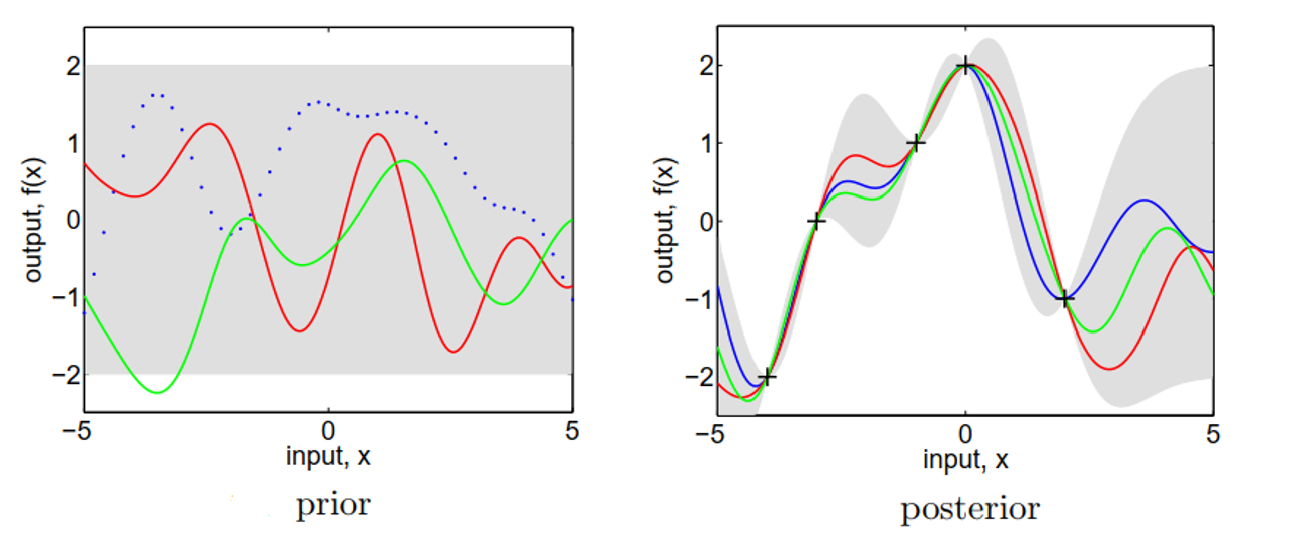
\includegraphics[width=12cm]{figs/prior-posterior.png}
\caption{The left figure shows three functions drawn at random from a GP prior. The dots indicate values of $y_{2,i}$ actually generated. The right figure depicts functions that have been drawn as lines by joining a large number evaluated pionts. Notice that the functions look smooth. The middle figure depicts three random functions drawn from the posterior. The + signs are five noise free observation indicated. In both plots the shaded area represents the pointwise mean $\mu_{1|2}$ plus and minus $2\sigma_{1|2}$ known as the 95 percent \textbf{confidence region}. Pay attention to the fact that the variance vanishes rapidly near the observed data points and increase as we get away from them. \cite{Rasmussen2006}.}
\label{fig:prior:posterior}
\end{figure}

\subsubsection{Noisy Prediction}
It is typical for more realistic modelling situations that we do not have access to function values themselves, but only noisy versions of them. Consequenlty, it is reasonabe to write
\begin{equation*}
\mathbf{Z}_{1} = \mathbf{Y}_{1} + \boldsymbol{\mathcal{E}},
\eqnum
\end{equation*}
where $\boldsymbol{\mathcal{E}}\in\mathbb{R}^n$ is a random noise vector. Assume that $\mathbf{Y}_1$ and $\boldsymbol{\mathcal{E}}$ are independent random vectors and that the noise random vector is Gaussian $p_{\boldsymbol{\mathcal{E}}}(\boldsymbol{\epsilon})=\mathcal{N}(\boldsymbol{\epsilon}; \mathbf{0}, \sigma_{\epsilon}\mathsf{I})$. It then follows that
 \begin{align*}
 \mathbb{E}(Z_{1,i}) &=  \mathbb{E}(Y_{1,i}) +  \mathbb{E}(\mathcal{E}_{1,i}) = 0 + 0 = 0, \\
 \cov(Z_{1,i},Z_{1,j}) &=  \cov(Y_{1,i},Y_{1,j}) +  \cov(\mathcal{E}_{i},\mathcal{E}_{j}) + 2 \cov(Y_{1,i},\mathcal{E}_{j}) = 
 \kappa(\mathbf{x}_{1,i}, \mathbf{x}_{1,j}) + \sigma_{\epsilon}^2\delta_{ij},
 \eqnum
 \end{align*}
where $\delta_{ij}$ is the Kronecker's delta. The first line follows from the linearity of expectation and the second line follows from bilinearity of the covariance and independence of $\mathbf{Y}_1$ and $\boldsymbol{\mathcal{E}}$. Futhermore, with a little bit of work, it can be shown that the associated joint PDF will be \cite[Sectoin 4.3]{Murphy2012}
\begin{equation*}
p_{\mathbf{Z}_{1}, \mathbf{Y}_{2}}(\mathbf{z}_{1}, \mathbf{y}_{2}) =
\mathcal{N} \left(
\begin{bmatrix}
\mathbf{z}_1 \\
\mathbf{y}_2
\end{bmatrix} ;
\begin{bmatrix}
\mathbf{0} \\
\mathbf{0}
\end{bmatrix} ,
\begin{bmatrix}
\mathsf{\Sigma}_{11}+\sigma_{\epsilon}^2\mathsf{I} & \mathsf{\Sigma}_{12} \\
\mathsf{\Sigma}_{21} & \mathsf{\Sigma}_{22} 
\end{bmatrix}
\right) \sim
\begin{bmatrix}
\mathbf{Z}_1 \\
\mathbf{Y}_2
\end{bmatrix}
\eqnum
\label{eq:GP:noise:joint}
\end{equation*}
and the predictive distribution becomes
\begin{equation*}
p_{\mathbf{Y}_2|\mathbf{Z}_1}(\mathbf{y}_2|\mathbf{z}_1) =
\mathcal{N}(\mathbf{y}_2; 
\mathsf{\Sigma}_{21}(\mathsf{\Sigma}_{11} + \sigma_{\epsilon}^2\mathsf{I})^{-1}\mathbf{z}_1, 
\mathsf{\Sigma}_{22} - \mathsf{\Sigma}_{21} (\mathsf{\Sigma}_{11}+\sigma_{\epsilon}^2\mathsf{I})^{-1} \mathsf{\Sigma}_{12}).
\eqnum
\label{eq:GP:posterior:noise}
\end{equation*}
In comparison with \cref{eq:GP:posterior}, we have replaced $\mathsf{\Sigma}_{11}$, $\mathbf{Y}_1$,  $\mathbf{y}_1$ with $\mathsf{\Sigma}_{11}+\sigma_{\epsilon}^2\mathsf{I}$,  $\mathbf{Z}_1$, $\mathbf{z}_1$, respectively.

\subsection{GP Algorithm}
Let us simplify our formulation of \cref{eq:GP:posterior:noise} a little bit. In the case that there is only one test point we introduce the following notation for the sub-blocks of the covariance matrix
\begin{equation*}
\mathsf{K}:=\mathsf{\Sigma}_{11} ,  \qquad
\mathbf{k}:=\mathsf{\Sigma}_{12}  =\mathsf{\Sigma}_{21}^{\top}, \qquad
k := \mathsf{\Sigma}_{22},
\eqnum
\end{equation*}
and the resulting simplifications follow
\begin{equation*}
\mathbf{Y}_2 = Y_2, \qquad
\mathbf{y}_2 = y_2, \qquad
\boldsymbol{\mu}_{1|2} = \mu_{1|2} \qquad
\mathsf{\Sigma}_{1|2} = \sigma_{1|2}.
\eqnum
\end{equation*}
Then, the posterior PDF in \cref{eq:GP:posterior:noise} reduces to a univariate Gaussian
\begin{equation*}
p_{Y_2|\mathbf{Y}_1}(y_2|\mathbf{y}_1) = 
\mathcal{N}(y_2; \mathbf{k}^{\top}(\mathsf{K} + \sigma_{\epsilon}^2\mathsf{I})^{-1}\mathbf{y}_1, k - 
\mathbf{k}^{\top} (\mathsf{K}+\sigma_{\epsilon}^2\mathsf{I})^{-1} \mathbf{k}),
\eqnum
\label{eq:GP:posterior:single}
\end{equation*}
and the posterior mean and variance will be
\begin{align*}
\mu_{1|2}  &= \mathbf{k}^{\top}(\mathsf{K}+\sigma_{\epsilon}^2\mathsf{I})^{-1}\mathbf{y}_1, \\
\sigma_{1|2} &= k - \mathbf{k}^{\top} (\mathsf{K}+\sigma_{\epsilon}^2\mathsf{I})^{-1} \mathbf{k}.
\eqnum
\end{align*}
Noting that $\mathsf{K}+\sigma_{\epsilon}^2\mathsf{I}$ is symmetric PD, using the Cholesky decomposition, we get $\mathsf{K}+\sigma_{\epsilon}^2\mathsf{I}=\mathsf{L}\mathsf{L}^{\top}$. Substituting this into the new formulation we obtain
\begin{align*}
\mu_{1|2}  &= \mathbf{k}^{\top}\mathsf{L}^{-\top}\mathsf{L}^{-1}\mathbf{y}_1, \\
\sigma_{1|2} &= k - (\mathsf{L}^{-1}\mathbf{k})^{\top}(\mathsf{L}^{-1}\mathbf{k}).
\eqnum
\label{eq:GP:posterior:alg}
\end{align*}
Using \cref{eq:GP:posterior:alg}, Algorithm \ref{alg:GP} addresses a simple method for calculating the predictive mean, variance, and hence the PDF in \eqref{eq:GP:posterior:single}.  It should be noted that we avoid computing the inverse directly as it is considered problematic from a numerical perpective \cite[Section 4.7]{Gill1991}. The main work is to compute the Cholesky decomposition, which takes $\mathcal{O}(\frac{1}{6}n^3)$ time. Solving the upper and lower-triangular linear systems in lines 14, 15, and 15 take $\mathcal{O}(\frac{1}{2}n^2)$ time. The dot produtcs in lines 16 and 19 needs $\mathcal{O}(n)$ time and the vector sum in line 19 requires $\mathcal{O}(n)$. Assuming that we use an SE kernel (RBF), calculating $\mathsf{K}$ takes a work of $\mathcal{O}(n^2d)$ and calculating $\mathbf{k}$ requires $\mathcal{O}(nd)$. Summing all these up, the running time $T(n,d)$ of the GP algorithm is of order
\begin{equation*}
T(n,d) \in \mathcal{O}\Big(\frac{1}{6}n^3+n^2d+\frac{3}{2}n^2+nd+n\Big),
\eqnum
\end{equation*}
where $n$ is the size of our dataset and $d$ is the number of features. In the case of $n \gg d$, this simplifies to
\begin{equation*}
T(n,d) \in \mathcal{O}\Big(\frac{1}{6}n^3\Big).
\eqnum
\end{equation*}
\begin{algorithm}[t!]
\caption{Gaussian Process}\label{alg:GP}
\hspace*{\algorithmicindent} {\scshape Input}: $\mathsf{X}_1, \, \mathbf{y}_1, \, \kappa, \sigma_{\epsilon}, \, \mathbf{x}_{2,1}$ \\
\hspace*{\algorithmicindent} {\scshape Output}: $\mu_{1|2}, \, \sigma_{1|2}$
\begin{algorithmic}[1]
\LineComment{Calculate $\mathsf{K}$.}
\For{$i=1$ \textbf{to} $n$}
    \For{$j=1$ \textbf{to} $n$}
        \State $\mathsf{K}_{ij} = \kappa(\mathbf{x}_{1,i},\mathbf{x}_{1,j})$;
    \EndFor
\EndFor
\LineComment{Calculate $\mathbf{k}$.}
\For{$i=1$ \textbf{to} $n$}
    \State $k_{i} = \kappa(\mathbf{x}_{1,i},\mathbf{x}_{2,1})$;
\EndFor
\LineComment{Calculate Cholesky decomposition.}
\State $\mathsf{L}=\text{Cholesky}(\mathsf{K}+\sigma_{\epsilon}^2\mathsf{I})$;
\LineComment{Calculate $\mu_{1|2}$.}
\State Solve $\mathsf{L} \mathbf{b} = \mathbf{y}_1$;
\State Solve $\mathsf{L}^{\top} \mathbf{a} = \mathbf{b}$;
\State $\mu_{1|2} = \mathbf{k}^{\top}\mathbf{a}$;
\LineComment{Calculate $\sigma_{1|2}$.}
\State Solve $\mathsf{L} \mathbf{c} = \mathbf{k}$;
\State $\sigma_{1|2}=k-\mathbf{c}^{\top}\mathbf{c}$;
\end{algorithmic}
\end{algorithm}

\subsection{Kernels and Hyperparameters}
Typically, the kernel functions that we use will have some free parameters, known as hyperparameters that are not determined during the learning process. According to eqs. \eqref{eq:RBF} and \eqref{eq:GP:posterior:single}, the hyperparameters for a noisy GP prediction with the SE kernel are the length-scale $\ell$, the signal variance $\sigma_y$, and the noise variance $\sigma_{\epsilon}$.  The hyperparameter $\sigma_y$ controls the amplitude of the covariance between the random variables $f(\mathbf{x})$ and $f(\mathbf{x}')$. $\sigma_{\epsilon}$ determines the amplitude of the variance of the noise $\mathcal{E}_i$. The hyperparameter $\ell$ determines a neighborhood radius around an input point $\mathbf{x}$ such that for every other input point $\mathbf{x}'$ lying in that neighborhood the corresponding random variables $f(\mathbf{x})$ and $f(\mathbf{x}')$ have a high correlation. Fig. \ref{fig:length:scale} illustrates the effect of this hyperparameter on the predictive distribution. The overall message of the figure is that the hyperparameters can significantly affect the posterior distribution. This gives rise to the question of how should we choose these hyperparameters. In the following, we address two methods for tunning hyperparameters, but this can be studied in more depth by consulting the Bible of GPs \cite[Chapter 5]{Rasmussen2006}.
\begin{figure}[t!]
\centering
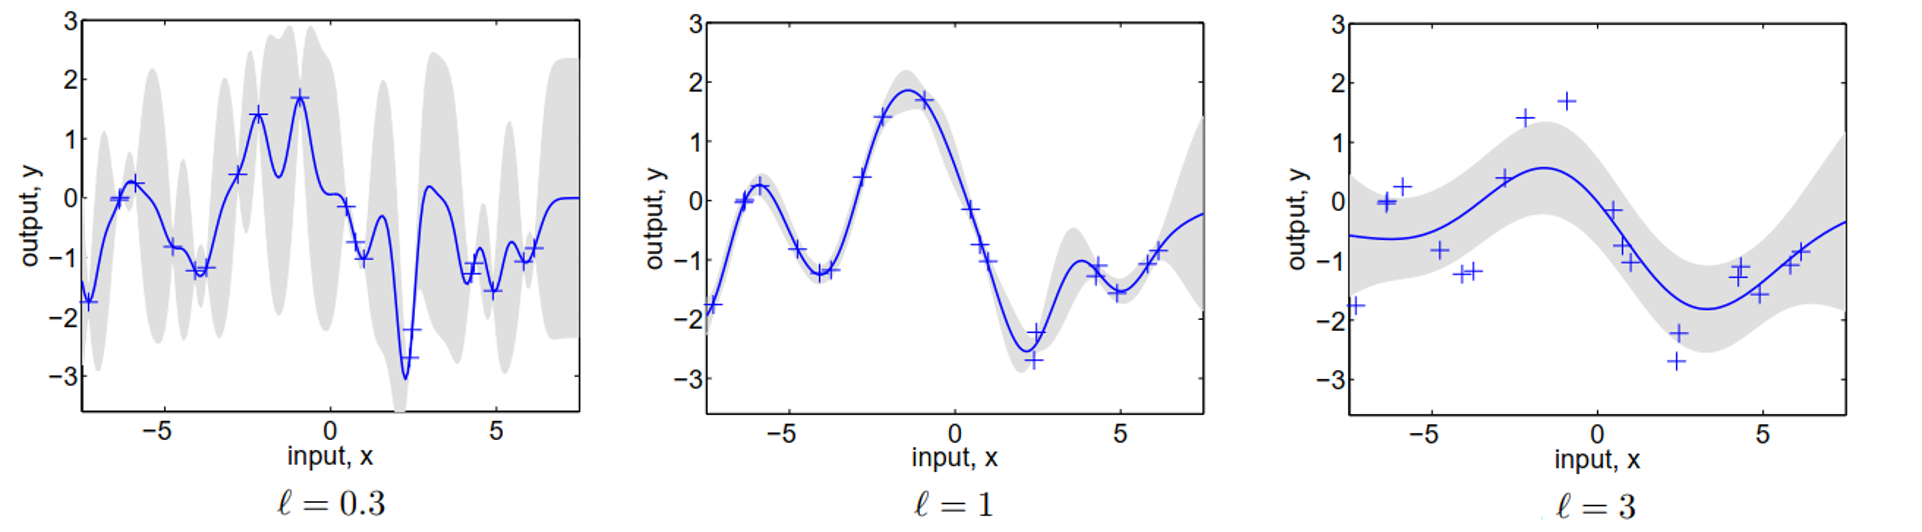
\includegraphics[width=17cm]{figs/length-scale.png}
\caption{In all three figures + signs show the training data and the solid blue line is the posterior mean. The figures show GPs with SE kernels but different hyper-parameters fit to 20 noisy observations. In the left figure, the hyperparameters are $(\ell, \sigma_y, \sigma_{\epsilon})=(0.3, 1.08, 0.00005)$ that corresponds to a short length-scale and as we see the wiggly looking mean oscillates so rapidly that it has fit almost all training data, ringing the bell for possible overfitting . In the middle figure, the hyperparameter are $(\ell, \sigma_y, \sigma_{\epsilon})=(1, 1, 0.1)$ that corresponds to a medium length-scale. The oscillations of the mean are reduced in comparison with the left figure. This is in agreement with our intuition that the length-scale represents a neighborhood radius that you can move in the input space before the target values change drastically. In the right figure, the hyper parameters are  $(\ell, \sigma_y, \sigma_{\epsilon})=(3, 1.16, 0.89)$, which corresponds to a long length-scale. As we see, the mean varies so slowly and has not fit many of the training data, showing that the model's bias has increased significantly. In all of the figures, if the $x$-axis were extended one would observe that the width of the confidence region $4\sigma_{1|2}$ remains constant and reaches the value $4\sigma_y$. You can get more sense about this phenomenon by looking at \cref{eq:GP:posterior:alg} \cite{Rasmussen2006}.}
\label{fig:length:scale}
\end{figure}

\subsubsection{Cross Validation}
In this sub-section, we consider how to use methods of cross-validation (CV) for determining hyperparameters. The basic idea is to split the training set into two disjoint sets, one which is actually used for training, and the other, the \textbf{validation set}, which is used to monitor performance, as shown in \cref{fig:cross:validation}. The performance on the validation set is used as a measure for the \textbf{generalization error} and determining hyperparameters is done based on this.
\begin{figure}[b!]
\centering
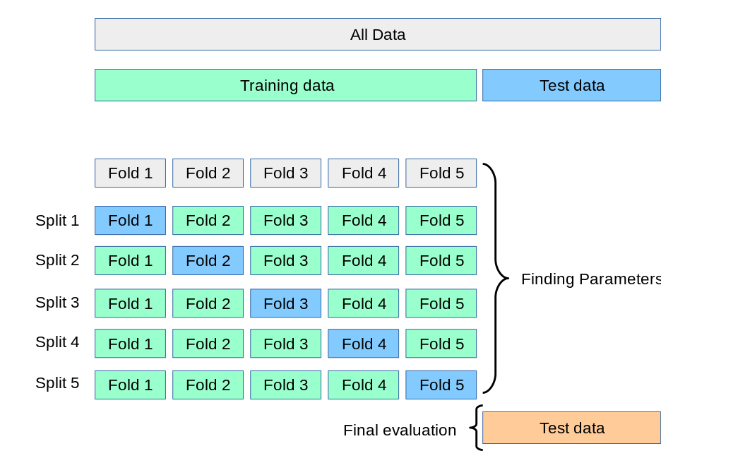
\includegraphics[width=9cm]{figs/cross-validation.png}
\caption{The figure illustrates a $5$-fold cross validation \cite{sklearn}.}
\label{fig:cross:validation}
\end{figure}
In practice a drawback of this method is that only a fraction of the full data set can be used for training, and that if the validation set is small, the performance estimate obtained may have large variance. To minimize these problems, CV is almost always used in the $k$-\textbf{fold} setting. In $k$-fold CV data is split into $k$ disjoint, equally sized subsets; validation is done on a single subset and training is done using the union of the remaining $k -1$ subsets, the entire procedure being repeated $k$ times, each time with a different subset for validation. Thus, a large fraction of the data can be used for training, and all cases appear as validation cases. The price is that $k$ models must be trained instead of one. Typical values for $k$ are in the range 3 to 10. An extreme case of $k$-fold cross-validation is obtained for $k = n$, the number of training data points, also known as \textbf{Leave-One-Out Cross-Validation} (LOO-CV). Often the computational cost of LOO-CV (training $n$ models) is high. Cross-validation can be used with any loss function. Although the \textbf{squared error loss} is by far the most common for regression \cite[Chapter 5]{Rasmussen2006}. 

To summarize, you should consider discrete values for each hyperparameter and construct a \textbf{search grid} for each split shown in \cref{fig:cross:validation}. Then, you calculate the squared error loss for each point of the grid in a fixed split. Repeating this for all of the splits, you obtain $k$ different squared error loss for each point of the grid. Finally, you can choose that value of the hyperparameters that results in the minimum averaged squared error loss over all the $k$ values.

\subsubsection{Marginal Likelihood}
\begin{figure}[t!]
\centering
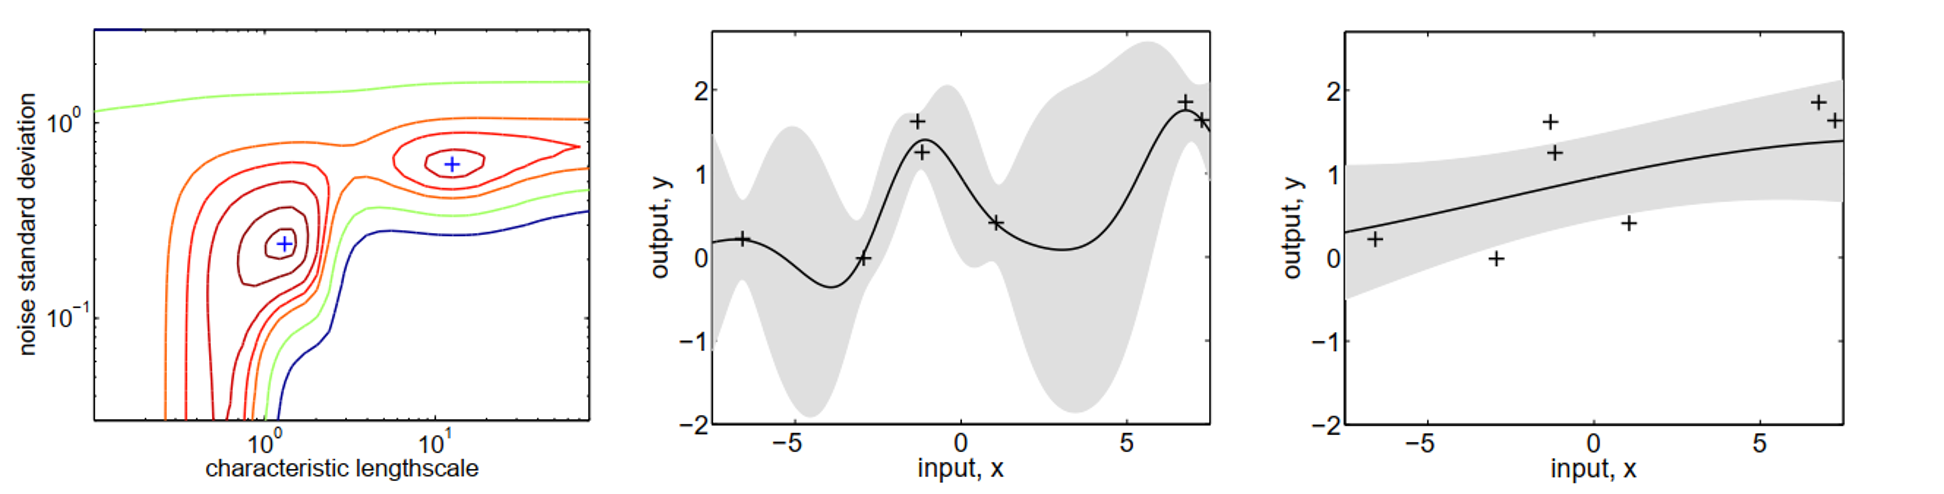
\includegraphics[width=17cm]{figs/marginal-likelihood.png}
\caption{The left figure shows the marginal likelihood as a function of the hyperparameters $\ell$ and $\sigma_{\epsilon}$. Signal's standard
deviation is chosen to be $\sigma_y^2 = 1$ for a dataset of 7 observations shown by + signs in the other two figures. There are two local optima, indicated with + signs in the left figure. The middle figure shows the function corresponding to the lower left local maximum that has the hyperparameters $(\ell, \sigma_{\epsilon}^2)=(1, 0.2)$ and is indeed the global maximum. This is quite \textit{wiggly} and has low noise and short length-scale. The function corresponding to the top right local maximum has the hyperparameters $(\ell, \sigma_{\epsilon}^2)=(10, 0.8)$. This is quite smooth and has high noise and long length-scale \cite[Section 5.4.1]{Rasmussen2006}. With only 7 data points, there is not enough evidence to confidently decide which is more reasonable, although the more oscillating model (middle figure) has a marginal likelihood that is about 60 percent higher than the simpler model (right figure)\cite[Section 15.2.4]{Murphy2012}.}
\label{fig:marginal:likelihood}
\end{figure}
In this method, we look for those hyperparameters that maximize the probability of seeing the training data, i.e. maximizing the marginal likelihood (ML) $p_{\mathbf{Z}_1}(\mathbf{z}_1)$. This is indeed based on the \textbf{frequentist} view of statistics. From \eqref{eq:GP:noise:joint}, we know that
\begin{equation*}
p_{\mathbf{Z}_1}(\mathbf{z}_1) = 
\mathcal{N}(\mathbf{z}_1; \mathbf{0}, \mathsf{\Sigma}+\sigma_{\epsilon}\mathsf{I}) = 
\mathcal{N}(\mathbf{z}_1; \mathbf{0}, \mathsf{K}_z),
\eqnum
\end{equation*}
where we have used the definition $\mathsf{K}_z:= \mathsf{K}+\sigma_{\epsilon}^2\mathsf{I}$. If we denote the vector of hyperparameters in a GP model by $\boldsymbol{\theta}\in\mathbb{R}^h$, then the ML method looks for the following maximizer
\begin{equation}
\boldsymbol{\theta^{*}} = \argmax_{\boldsymbol{\theta}\in\mathbb{R}^h} p_{\mathbf{Z}_1}(\mathbf{z}_1; \boldsymbol{\theta}) =   
\argmax_{\boldsymbol{\theta}\in\mathbb{R}^h} \log p_{\mathbf{Z}_1}(\mathbf{z}_1; \boldsymbol{\theta}),
\eqnum
\label{eq:marginal}
\end{equation}
where the second equality follows because the natural logrithm is an strictly increasing function and does not change the optimizer. The term \textit{marginal} refer to the fact that the likelihood $p_{\mathbf{Z}_1}(\mathbf{z}_1;\theta)$ can be obtained by perfoming marginalization on the PDF given in \eqref{eq:GP:noise:joint}. This is sometimes refered as \textbf{emprical Bayes} since pure Baysians believe that this method is fallacious. They argue that when we solve the optimization problem in \eqref{eq:marginal} then the hyperparameters $\boldsymbol{\theta}$ will depend on the seen data $\mathbf{y}_1$; however, all of our calculation was based on the fact that they are independent of the observed data \cite[Lecture 9]{Freitas2013}. For this reason, more complicated methods such as Monte Carlo (MC) methods have been developed to optimize the hyperparametrs \cite[Section 45.5]{MacKay2003}. With this in mind, ML is usually done in practice and the numerical results are satisfactory. 

To solve the nonlineaer unconstrained optimization problem in \cref{eq:marginal}, one needs to calculate the gradient. Feeding the result into any gradient solver for such problems could find the solution. According to \eqref{eq:GP:noise:joint}, natural logarithm of the ML (log-ML) will be
\begin{equation*}
\log p_{\mathbf{Z}_1}(\mathbf{z}_1;\theta) = 
\log\mathcal{N}(\mathbf{z}_1;\mathbf{0}, \mathsf{K}_z) =
-\frac{1}{2}\mathbf{z}_1^{\top}\mathsf{K}_z^{-1}\mathbf{z}_1-\frac{1}{2}\log\det\mathsf{K}_z-\frac{n}{2}\log2\pi,
\eqnum
\label{eq:ML:log}
\end{equation*}
To calculate the gradient, we need the following lemma
\begin{lem}
Suppose that $\mathsf{K}(\boldsymbol{\theta})\in\mathbb{R}^{n,n}$ is an invertible matrix whose elements depend on the vector $\boldsymbol{\theta}\in\mathbb{R}^h$. The the following matrix derivative identities are valid
\begin{equation*}
\partial_{\theta_i} \mathsf{K}^{-1} = - \mathsf{K}^{-1}\partial_{\theta_i}\mathsf{K}\,\,\mathsf{K}^{-1}, \qquad
\partial_{\theta_i}\log\det\mathsf{K} = \tr(\mathsf{K}^{-1}\partial_{\theta_i}\mathsf{K}), \qquad
i=1,\dots,h,
\eqnum
\label{eq:matrix:der}
\end{equation*}
where $\partial_{\theta_i} \mathsf{K}$ is an elementwize derivative with respect to $\theta_i$ and $\tr$ is the trace of a matrix.
\end{lem}
Using \cref{eq:matrix:der}, computing the gradient of log-ML in \cref{eq:ML:log} leads to
\begin{align*}
\partial_{\theta_i}\log p_{\mathbf{Z}_1}(\mathbf{z}_1;\theta) &= 
\frac{1}{2}\mathbf{z}_1^{\top}\mathsf{K}_z^{-1}\partial_{\theta_i}\mathsf{K}_z\,\,\mathsf{K}_z^{-1}\mathbf{z}_1 - 
\frac{1}{2} \tr(\mathsf{K}_z^{-1}\partial_{\theta_i}\mathsf{K}_z) \\
&= \frac{1}{2}\mathbf{a}^{\top}\partial_{\theta_i}\mathsf{K}_z\,\,\mathbf{a} - \frac{1}{2} \tr(\mathsf{K}_z^{-1}\partial_{\theta_i}\mathsf{K}_z) \\
&= \frac{1}{2}\tr(\mathbf{a}^{\top}\partial_{\theta_i}\mathsf{K}_z\,\,\mathbf{a}) - \frac{1}{2} \tr(\mathsf{K}_z^{-1}\partial_{\theta_i}\mathsf{K}_z) \\
&= \frac{1}{2}\tr(\mathbf{a}\mathbf{a}^{\top}\partial_{\theta_i}\mathsf{K}_z) - \frac{1}{2} \tr(\mathsf{K}_z^{-1}\partial_{\theta_i}\mathsf{K}_z) \\
&= \frac{1}{2}\tr((\mathbf{a}\mathbf{a}^{\top}-\mathsf{K}_z^{-1})\partial_{\theta_i}\mathsf{K}_z), \\
&= \frac{1}{2}\tr\Big(\big((\mathsf{K}_z^{-1}\mathbf{z}_1)(\mathsf{K}_z^{-1}\mathbf{z}_1)^{\top}-\mathsf{K}_z^{-1}\big)\partial_{\theta_i}\mathsf{K}_z\Big),
\eqnum
\label{eq:ML:log:grad}
\end{align*}
where we used the fact that the trace of a scalar equals the scalar itself along with the linearity of the trace and the general identity $\tr(\mathsf{A}\mathsf{B})=\tr(\mathsf{B}\mathsf{A})$. The computational cost for the ML in \eqref{eq:ML:log:grad} is dominated by computing the inverse $\mathsf{K}_z^{-1}$. More specifically, since $\mathsf{K}_z$ is symmetric PD, its inverse can be computed by first calculating the Cholesky decomposition and solving $n$ resulting upper- and lower-triangular linear systems, which takes a work of $\mathcal{O}(n^3)$.

Fig. \ref{fig:marginal:likelihood} illustrates an example of finiding the optimal values for hyperparameters $\boldsymbol{\theta}=(\ell, \sigma_{\epsilon})^{\top}$ of a GP model with an SE kernel. We observe that there may exist several local optimums as the marginal likelihood is not a convex function.

\subsubsection{Constructing New Kernels}
As described earlier, the power of GP lies in the choice of the kernel function. This property allows us to introduce domain knowledge into the process and lends GPs their flexibility to capture trends in the training data. For example, by choosing a suitable length-scale for the RBF kernel, we can control how smooth and oscillating the resulting function will be. A big benefit that kernels provide is that they can be combined together, resulting in a more specialized kernel. The decision of which kernel to use is highly dependent on prior knowledge about the data, e.g. if certain characteristics are expected \cite{Gortler2019}.

The only constraint on our choice of covariance function is that it must generate a PD covariance matrix for any set of input points. In this connection, we have following theorem
\begin{thm}
The sum and product of two kernels is a kernel.
\end{thm}
For the proof of this theorem, a wide range of kernel functions, and other possibilities of combining kernels see \cite[Section 4.2]{Rasmussen2006}. For example, the sum property can be used to add RBF kernels with different characteristic length-scales and product rule can be employed to produce trending functions with varying oscillations.
\begin{figure}[t!]
\centering
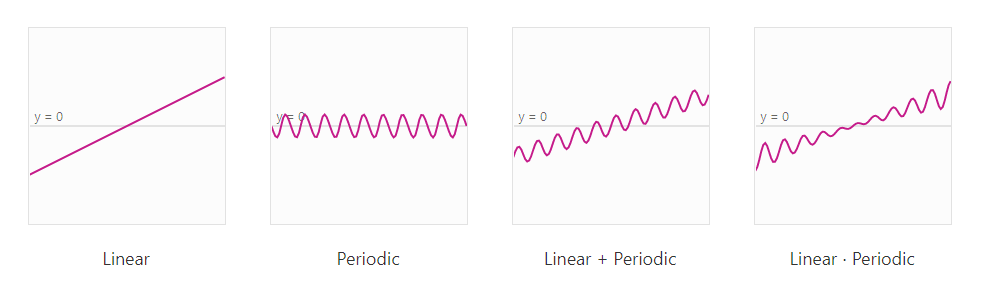
\includegraphics[width=17cm]{figs/combine-kernels.png}
\caption{The figures show samples drawn from prior distributions with different kernels. Addition results in an oscillating function with a global trend, while multiplication increases the oscillation amplitude outwards \cite{Gortler2019}.}
\label{fig:kernels:combine}
\end{figure}

Fig. \ref{fig:kernels:combine} depicts combinations of a linear and a periodic kernel via summation and multiplication. The two aforementioned kernels are defined as
\begin{align*}
\kappa_{\text{per}}(x,x') &= \sigma_y\exp\Big(-\frac{2}{\ell^2}\sin^2\Big(\frac{\pi( x-x')}{p}\Big)\Big), \\
\kappa_{\text{lin}}(x, x') &= \sigma_b+\sigma_y(x-c)^{\top}(x'-c),
\eqnum
\end{align*}
where $(\ell, \sigma_y, p)$ are the hyperparameters of the periodic kernel and $(\sigma_b, \sigma_y, c)$ are hyperparameters of the linear kernel. For more general forms of these kernel functions in higher dimensional input spaces see \cite[Section 45.4]{MacKay2003}.
\subsection{A Real World Example}
Here, we mention an interesting real world example of GPs in action. The computer graphics and animation fields are filled with applications that require the setting of tricky parameters. In many cases, the models are complex and the parameters are unintuitive for non-experts. \citeauthor{Brochu2010} \cite{Brochu2010} present an optimization method for setting parameters of a procedural fluid animation system by showing the user examples of different parametrized animations and asking for feedback. They simulate the fluid flow by taking the curl of a vector valued potential function which has several technical parameters. In this example, the the aforementioned parameters are the inputs $\mathbf{x}$ and the targets $\mathbf{y}$ are the feedbacks of the user and some previous default data. By introducing an \textbf{active learning} method, they employ the Bayesian technique of bringing in prior belief based on previous runs of the system and expert knowledge to assist users find good parameter settings in as few steps as possible. At the heart of the machinary they have produced, lies the GP introduced in this tutorial. The main benefit is that the GP helps construct an efficient \textbf{explore and exploit} strategy in the input space based on the distribution of uncertainty in that space \cite[Lecture 9]{Freitas2013}. Watch the video of the \textbf{interactive interface} they have created to help users create animations without taking the burdon of adjusting parameters manually \cite{Brochu2010Animation}. Indeed, this idea is not restericted to computer graphics field and can be employed anywhere else that requires the adjusment of techincal parameters.


\section{What is Next?}
In this tutorial, we took a trip from the basics of GPs to their real world applications. We learned that GPs are \textbf{supervised probabilistic} models with high capability for doing regression. Fortunately, they can also be extended for classification tasks. For this purpose, the main idea is to pass the output values  through a sigmoid function. You can study more about this in \cite[Chapter 3]{Rasmussen2006}. More surprisingly, GPs have several models as their special cases. Indeed, some of the well known results are that
\begin{enumerate}[noitemsep]
\item Using \cref{eq:GP:posterior:alg} and Mercer's theorem \cite[Section 4.3]{Rasmussen2006}, it can be shown that the posterior mean $\mu_{1|2}$ is equivalent to a Regression model with nonlinear basis functions and \textbf{inifinite} number of parameters. In this regard, it is said that a GP model is a \textbf{non-parametric} model. Despite what the name suggests, it is meant that it can have as many parameters as required.
\item The Ridge regression model can be recoverd by the posterior mean $\mu_{1|2}$, if we choose a dot product kernel $\kappa(\mathbf{x},\mathbf{x}')=\mathbf{x}^{\top}\mathbf{x}'$ and set the noise variance $\sigma_{\epsilon}$ equal to the regularization parameter $\delta$ \cite[Lecture 9]{Freitas2013}.
\item It can also be shown that specific large neural networks are equivalent to a GP \cite{MacKay1998}.
\end{enumerate}
The main drawback of GPs is their $\mathcal{O}(n^3)$ time complexity, which makes it hard to scale. One of the main trends of research in recent years is to make GPs appropriate for large datasets. You can start reading about this in \cite[Chapter 8]{Rasmussen2006}. A good review about scalable GPs is also presented in \cite{Liu2020}.


\section{Support}
I am happy that you have read this so far, showing that you are serious about understanding GPs and machine learning. I tried to write an easy-to-follow and at the same time rigorous introduction to GPs and I hope that it appealed to you. If you liked this tutorial, please give the repository of this document a star on \href{https://github.com/Hosein-Rahnama/Gaussian-Processes.git}{GitHub}. Futhermore, you are more than welcomed to report any errors by opening an issue or to suggest further improvements by making pull requests on \href{https://github.com/Hosein-Rahnama/Gaussian-Processes.git}{GitHub}.


\newpage
\section{References}
\printbibliography[heading=none]

\end{document}